\label{sec:intro}


本文探索了能够处理3D几何数据比如点云和网格的深度学习模型。为了实现权重分享和其他核函数优化,典型的卷积结构要求输入数据的格式高度规则,比如图形网格和3D体素。由于点云或网格并不是有序格式,大多数研究人员通常会将这些数据转换为常规的3D体素或图像集合(例如视图),然后再将它们输入到深层网络中。然而,这种数据表示转换会使结果数据变不必要的大量增加,同时也会引入能模糊数据自然不变性的量化伪影。

因此我们重点介绍一种不同于以往只使用简单点云的3D几何神经网络,并将其命名为PointNets。点云是简单且统一的结构,能够避免网格的组合不规则性和复杂性,因此更容易学习。然而,PointNet依旧受限于点云只是点的一个集合这样一个事实,因此其内部元素的排列是不变的,需要在网络计算中做一些对称性处理。而更进一步的刚性运动的不变性也需要考虑。

我们构建的PointNet是一个统一的架构,这体现在将点云作为输入,输出整体输入或相对于输入的部分点块的类标签。该模型的基础构架非常的简单,因为在初始阶段,每个点的处理方法完全相同且独立。在基础设置中,每个点仅用它的三个坐标(x,y,z)来表示。额外维度可以通过计算法线和其他局部或者全局特征来添加得到。

我们这个方法的关键在于使用对称的max pooling函数。网络有效地学习一组优化函数/准则,从点云中选择感兴趣的点或者含有信息的点,并编码选择的原因。网络最终的全连接层把这些学习到的最优值聚合到如上所述的整个形状的全局描述符(形状分类)上或者用于预测每个点标签(形状分割)。

我们的输入格式很容易应用刚性或者仿射变换,因为每个点都是独立变换的。因此我们可以在应用PointNet处理点云之前添加一个与数据无关的空间转换网络来规范化点云数据,以此来进一步提高结果的表现。

我们提供了方法的理论分析和实验评估,展示了我们的网路可以近似任何连续的集合函数。更有趣的是,事实证明我们的网络通过学习一组稀疏的关键点来概括一个输入点云,这些关键点根据可视化结果在视觉上大致对应对象的骨架。理论分析解释了为什么我们的PointNet对于输入点云的微小扰动,以及由极端点插入或删除点带来的数据损坏有着良好的健壮性。

我们对大量参照数据集(包括形状分类、零件分割、场景分割)进行实验,比较了PointNet和目前基于多视角与体积表示的最先进的方法。在统一的构架下,PointNet不仅在速度上更快,同时也表现出了和现有技术相当甚至更好的性能。
我们工作的主要贡献如下:
\begin{itemize}
    \item 我们设计了一个适用于处理3D无序点集的新型深度网络模型
    \item 我们展示了如何训练这样的网络模型来处理3D形状分类、零件分割和场景语义分析等任务
    \item 我们从实验和理论的角度分析了方法的稳定性和效率
    \item 我们演示了网络中所选择神经元计算出的3D特征,并对其性能进行了直观的解释
    
\end{itemize}
使用神经网络处理无序集合的问题是一个非常普遍和根本的问题,我们希望我们的想法也可以应用到其他领域。


\begin{figure}
    \centering
    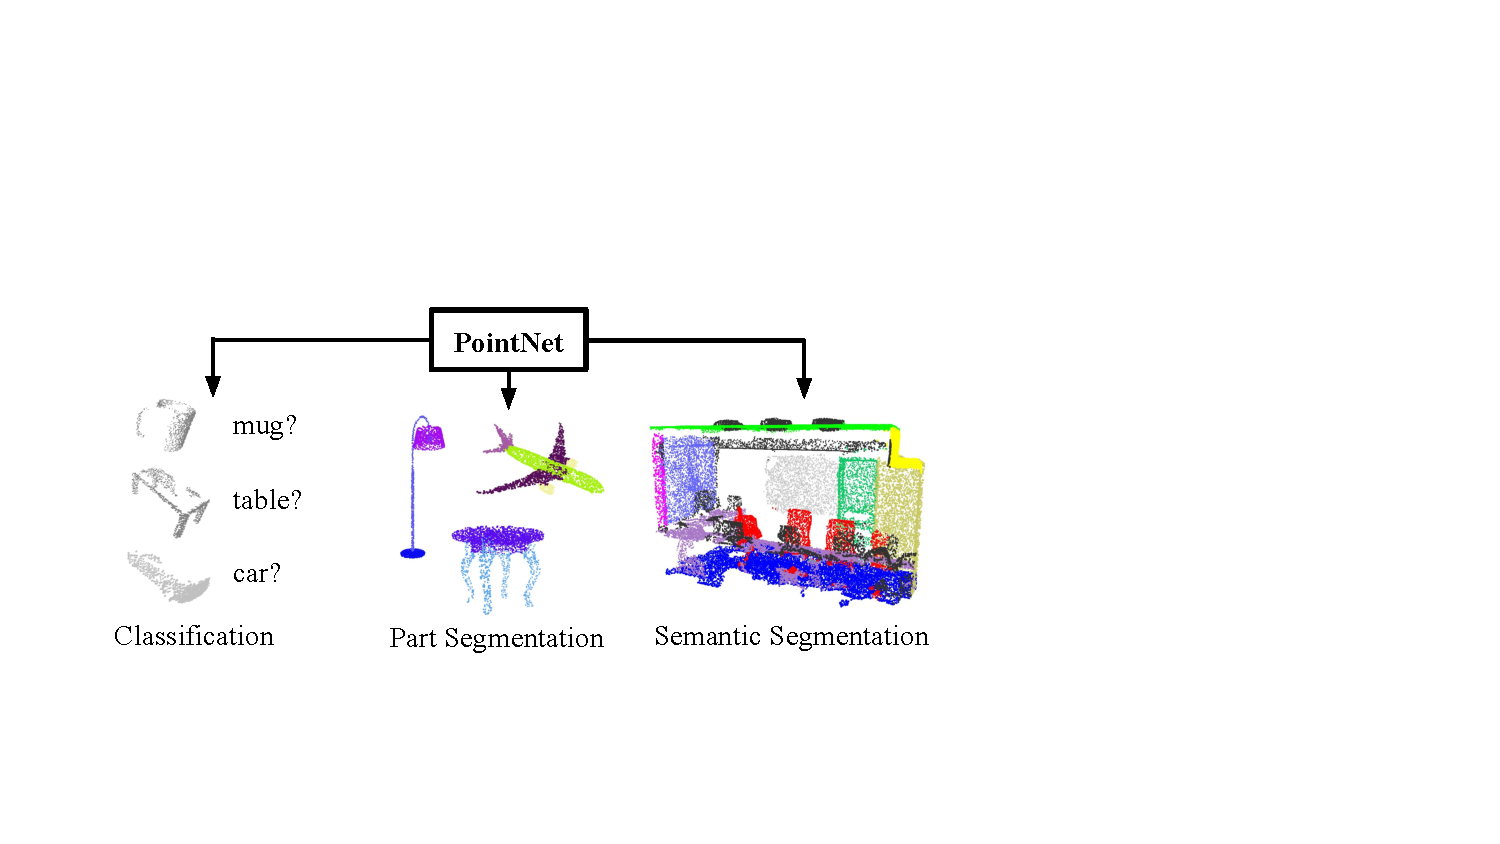
\includegraphics[width=\linewidth]{fig/teaser.pdf}
    \caption{\textbf{PointNet 的应用} 
    我们提出了一个新的神经网络结构,其输入为一个原始的点云(点的集合),没有经过体素化或预渲染。该网络具有一个统一的架构,能够学习全局和局部的点特征,从而为各种三维识别任务提供了一个简单、高速而有效的方法。 
    %We propose a novel deep net architecture that consumes raw point cloud (set of points) without voxelization or rendering. It is a unified architecture that learns both global and local point features, providing a simple, efficient and effective approach for a number of 3D recognition tasks.% 
    }
    \label{fig:teaser}
\end{figure}


\begin{figure*}[th!]
    \centering
    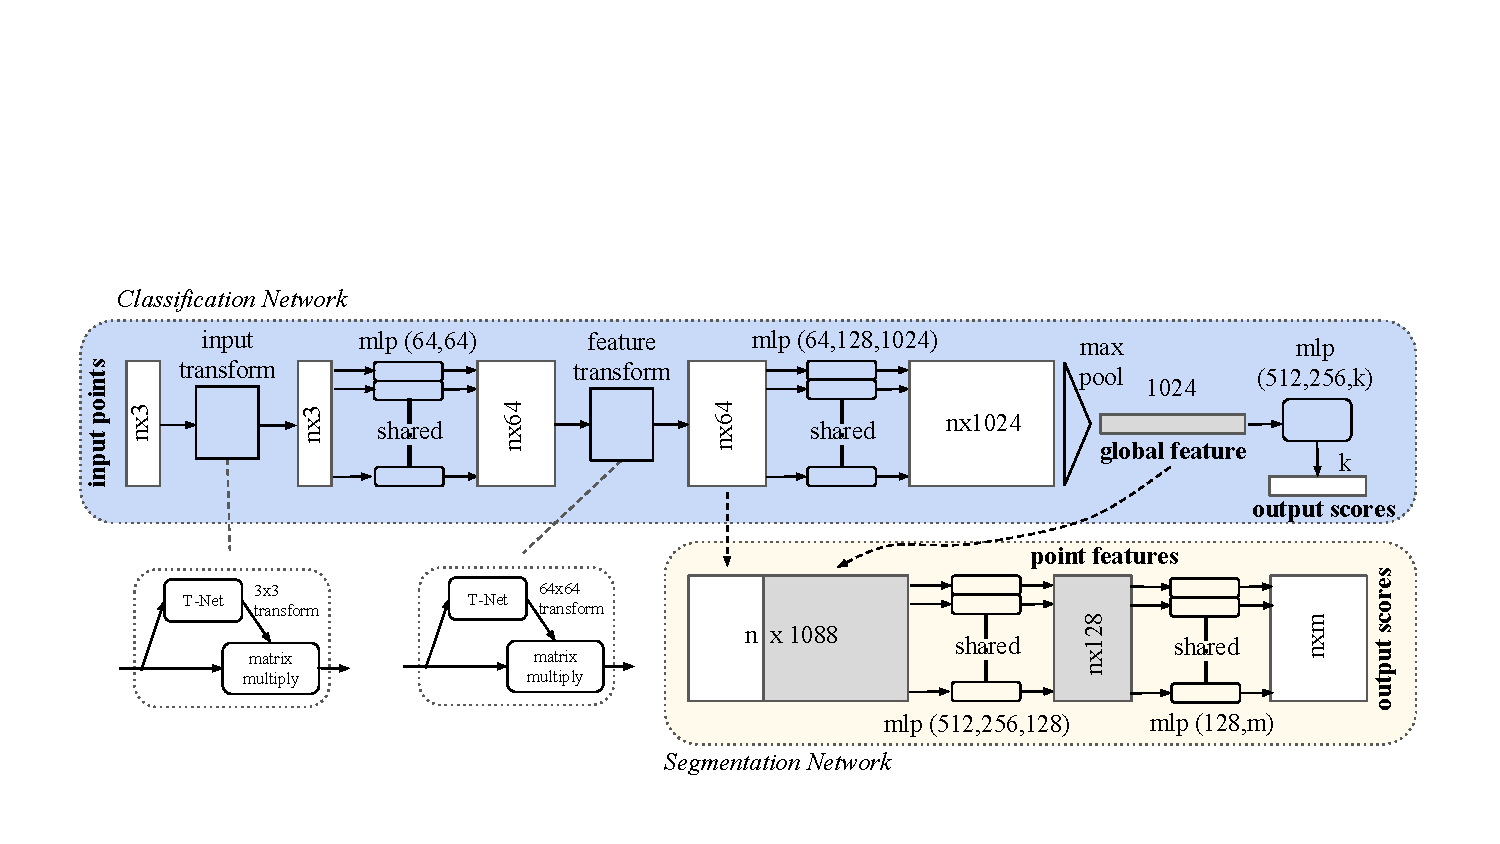
\includegraphics[width=0.9\linewidth]{fig/pointnet_fixed.pdf}
    \caption{\textbf{PointNet 架构}      分类网络将$n$个点作为输入,作用输入和特征变换,然后通过max pooling聚合点的特征,输出的是$k$种分类的分类分数。分割网络是分类网络的拓展,它连接局部和全局特征以及每个点输出的分数。``mlp''代表多层感知机,括号中的数字是层的大小。Batchnorm用于所有应用了ReLU的层。Dropout用于分类网络中的最后一个多层感知机。}
    \label{fig:pointnet_arch}
\end{figure*}